\documentclass[conference]{IEEEtran}
\IEEEoverridecommandlockouts
\usepackage{cite}
\usepackage{amsmath,amssymb,amsfonts}
\usepackage{graphicx}
\usepackage{textcomp}
\usepackage{xcolor}
\usepackage{subfigure}
\usepackage{booktabs}
\usepackage{multirow}
\usepackage[ruled,vlined]{algorithm2e}

\def\BibTeX{{\rm B\kern-.05em{\sc i\kern-.025em b}\kern-.08em
    T\kern-.1667em\lower.7ex\hbox{E}\kern-.125emX}}
\begin{document}

\title{Coordination of Virtual and Physical Multiple Vehicles: A Digital Twin Realization Method}
	

\author{\IEEEauthorblockN{1\textsuperscript{st} Chunying Yang}
	\IEEEauthorblockA{\textit{School of Vehicle and Mobility} \\
		\textit{Tsinghua University}\\
		Beijing, China \\
		ycyacademic@gmail.com}
	\and
	\IEEEauthorblockN{2\textsuperscript{nd} Qing Xu}
	\IEEEauthorblockA{\textit{School of Vehicle and Mobility} \\
		\textit{Tsinghua University}\\
		Beijing, China \\
		qingxu@tsinghua.edu.cn}
	\and
	\IEEEauthorblockN{3\textsuperscript{rd} Jianghong Dong}
	\IEEEauthorblockA{\textit{School of Vehicle and Mobility} \\
		\textit{Tsinghua University}\\
		Beijing, China \\
		18801380768@163.com}
	\and
	\IEEEauthorblockN{4\textsuperscript{th} Mengchi Cai}
	\IEEEauthorblockA{\textit{School of Vehicle and Mobility} \\
		\textit{Tsinghua University}\\
		Beijing, China \\
		cmc18@mails.tsinghua.edu.cn}
	\and
	\IEEEauthorblockN{5\textsuperscript{th} Hongmao Qin}
	\IEEEauthorblockA{\textit{Wuxi Intelligent Control Research Institute,HNU} \\
		\textit{Hunan University}\\
		Wuxi, China \\
		qinhongmao@hnu. edu. cn}
	\and
	\IEEEauthorblockN{6\textsuperscript{th} Jianqiang Wang}
	\IEEEauthorblockA{\textit{School of Vehicle and Mobility} \\
		\textit{Tsinghua University}\\
		Beijing, China \\
		wjqlws@tsinghua.edu.cn}
	\and
	\IEEEauthorblockN{7\textsuperscript{th} Keqiang Li}
	\IEEEauthorblockA{\textit{School of Vehicle and Mobility} \\
		\textit{Tsinghua University}\\
		Beijing, China \\
		likq@tsinghua.edu.cn}
}
\maketitle

\begin{abstract}
	In the last few years, theories and applications of digital twin (DT) have experienced explosive growth. To conduct field implementation of multiple vehicle coordination, we develops a system called DIRS under digital twin paradigm, which contains physical space, cyber space and cloud. Especially, the combination of physical and virtual vehicles enables field validation even under circumstance that the number of accessible physical vehicles is insufficient. To demonstrate system performance, we conduct several experiments in platoon scenario and analyze results in terms of safety and mobility.
\end{abstract}

\begin{IEEEkeywords}
	Digital twin, multi-vehicle cooperative control, field validation 
\end{IEEEkeywords}
\section{Introduction}
	Digital twin (DT), an emerging representation of cyber-physical systems, has attracted increasing attentions recently. It opens the way to real-time monitoring and synchronization of real-world activities with the virtual counterparts\cite{ref:intro1}. In the field of simulation of Connected and Automated Vehicles (CAVs), related theories and applications have experienced explosive growth in the last several years because of its unique features. Compared to traditional simulation methods, DT paradigm has the following advantages. First, relying on reliable communication and sensor technology, DT system can access real-time data from physical world during running process. Second, since DT paradigm emphasizes two-way interaction between physical and cyber spaces, it is realizable for physical entities to receive feedback from cyber space at a very high frequency to achieve status updates. \cite{ref:intro1} proposed a general framework of DT system for connected vehicles, which is the first combination of DT and CAVs. \cite{ref:intro2} used a DT approach to develop a cooperative ramp merging system and conducted field implementation. Also, they evaluated system effectiveness in terms of mobility and fuel consumption.
	
	With the development of V2X communication, coordinated control of multiple vehicles has been widely studied. \cite{ref:lfq} proposed a unified multi-vehicle formation control framework for CAVs, and they combined SUMO and Matlab to verify its functions. \cite{ref:ccy} presented a graph-based vehicle cooperation method to guarantee safety and efficiency at unsignalized intersections. However, field experiment is rarely implemented due to high expenses and demand for extra-large space. Therefore, most researches of multi-vehicle coordination use simulation to deploy, validate and compare impacts of their algorithms on coordination tasks of CAVs. 
	
	Conducting field experiment of multi-vehicle coordination using a DT method seems to be a feasible solution. Relying on two-way interaction between physical and cyber spaces and several real vehicles, it is possible to perform coordination tasks even the number of real vehicles is insufficient. \cite{ref:intro3} proposed a trajectory-following guidance method to chase a virtual target, which inspired method proposed by this study that field experiment of multiple vehicles coordination can be conducted with several real vehicles (or physical vehicles) and a group of virtual vehicles existing in cyber space.
	
	Compared to other recent study on DT system realization and field validation of multi-vehicle coordination algorithms, this study has the following major contributions:
	\begin{itemize}
		\item To our knowledge, this study is the first to propose implementing field validation of multiple vehicles coordination algorithms using a DT method. Moreover, this study designs and develops a realization system to conduct field experiment even the number of accessible vehicles is insufficient.   
		\item The system offers various ways to support human-machine interaction. For instance, a mixed reality device (Hololens) is leveraged to visualize cyber space and trigger sudden events. Besides, a driving simulator is incorporated to demonstrate driver's perspective.
	\end{itemize}
	
	The remainder of this paper is organized as follows. Section~\ref{sec:methodology} introduces the realization system in detail, including architecture and components, interaction designing and hierarchical mechanism of vehicle control. In section~\ref{sec:simulation}, we reveals a case study for platooning scenario and presents the experiment results. The last section concludes this article and shows a prospect of this work. 
	
\section{Methodology}
\label{sec:methodology}
	In this study, we designs and develops a CAVs-orientated digital twin realization system (DIRS) in Tsinghua university, which supports field validation of multiple vehicles coordination methods. To meet such a purpose, this study proposes using combination of physical and virtual vehicles to execute coordination tasks. Specifically, DIRS models two kinds of vehicles in cyber space. One of them is called twin vehicle, which is used to exhibit real-time running status of corresponding physical counterpart, and the other is called cloud vehicle, which is used to simulate behaviors of physical vehicles. Interactions between twin vehicle and cloud vehicle, in turn, can influence decisions and behaviors of physical vehicles. The fact that field experiments of coordination tasks are barely conducted is mainly attributed to financial and safety considerations. However, DIRS seems to be a solution. The combination of physical and virtual vehicles makes it possible to implement field testing even the number of accessible real vehicles is inadequate.
	
	In the section that follow we describe DIRS in more technical detail, providing overviews of architecture and components, human-machine interaction designing and hierarchical mechanism of vehicle controlling.
\subsection{System architecture and components}
	\begin{figure}[htbp]
		\centering
		\includegraphics[width=.48\textwidth]{figure/systemArchitecture.png}
		\caption{System architecture}
		\label{fig:systemArchitecture}
	\end{figure}
	A schematic overview of system architecture is depicted in Fig.~\ref{fig:systemArchitecture}. DIRS is composed of three major components\,--\,physical space, which is in the form of sand table testbed, cyber space and cloud, among which cloud functions as information integration center that links the other two components.

\par\textbf{Physical Space}:

	In digital twin paradigm, physical space of DIRS refers to a sand table testbed as shown in Fig. \ref{fig:sandTable}, which is equipped with miniature vehicles and traffic infrastructures and provides rich environment settings to support field testing.
	
	To achieve mapping from physical to cyber space, vehicle, which is key element of the system and thus is selected to explain its realization process. It should be noted that we assume vehicles are running on a flat surface without height variation for purpose of simplifying computation. Therefore, state parameters of vehicles are composed of position, orientation and speed. 
	
	Vision system composed of four overhead cameras is adopted to implement localization and orientation measurement considering relatively stable light conditions of the sand table. Fig.~\ref{fig:cameraCoverage} presents coverage of the vision system. Several steps are required to realize image-based status determination:
	\begin{itemize}
		\item \textbf{Distortion correction}
		\item \textbf{Identifying colors recognition}\\
		Colored blocks with unique combination are attached on the top of individual vehicle and are used to determine real-time running status. Fig \ref{fig:coloredVehicle} demonstrates vehicles with identifying colored blocks.
		\item \textbf{Coordinate transformation}
	\end{itemize}

	Due to word limitation, more details about these steps are uploads to our system website\cite{ref:website}.
 \begin{figure}[htbp]
 	\begin{centering}
 		\subfigure[]{
 			\includegraphics[width=0.14\textwidth]{figure/cameraCoverage.png}
 			\label{fig:cameraCoverage}}
 		\subfigure[]{
 			\includegraphics[width=0.14\textwidth]{figure/vehicle.JPG}
 			\label{fig:vehicle}}
 		\subfigure[]{
 			\includegraphics[width=0.14\textwidth]{figure/coloresVehicle.jpg}
 			\label{fig:coloredVehicle}}
 	\end{centering}
 	\caption {Physical space. (a) Camera coverage.  White, orange and green parallelograms represent area covered by one, two and four cameras respectively in order to guarantee seamless detection. (b) Miniature vehicle used by DIRS. (c) Vehicles with identifying colored blocks on the top}
 \end{figure}
 \begin{table}
 	\centering
 	\caption {Important parameters of physical space}
 	\label {tab:summarize}
 	\begin{tabular}{|c|c|c|}
 		\hline
 		\textbf{Parameters}&\textbf{Value}&\textbf{Unit} \\
 		\hline
 		Length of sand table&9&m\\
 		\hline
 		Width of sand table&5&m\\
 		\hline
 		Mass of miniature vehicle&1.4&Kg\\
 		\hline
 		Chassis size&200$\times$180$\times$130&mm\\
 		\hline
 		Maximum speed&1&m/s\\
 		\hline
 		Positioning error of X-axis&$\pm$6&mm\\
 		\hline
 		Positioning error of Y-axis&$\pm$3&mm\\
 		\hline
 		Mapping error of X-axis&$\pm$3&cm\\
 		\hline
 		Mapping error of Y-axis&$\pm$5&cm\\
 		\hline
 		Mapping error of heading&$\pm$2&degree\\
 		\hline
 		Image resolution&1920$\times$1080&Pixels per inch(PPI)\\
 		\hline
 		fps&30&\\
 		\hline
 	\end{tabular}
 \end{table}	 
 \par\textbf{Cyber Space}:
 
 	\cite{ref:taofei} proposed "Five-dimension model for the DT" and thought cyber space should support simulation, decision making and controlling of its corresponding physical space. When it comes to DIRS, we build cyber space with specific properties in mind. First, giving that open control parameters of miniature vehicles contain speed and steering only, which is insufficient in many cases. As a result, we model vehicles of cyber space with specific kinematics characteristics and other parameters. Second, we desire to visualize cyber space in a intuitional and immersive way. Since game engine is provided with excellent ability of scene rendering and high fidelity, it is adopted by many studies to construct cyber space recently, like \cite{ref:engine1,ref:engine2}. In this study, Unity3D (or Unity) is chosen because of its abundant asset resources and support for mixed reality development. Cyber space built with Unity is demonstrated as Fig.~\ref{fig:cyberSpaceUnity}. Compared to\cite{ref:taofei}, cyber space of DIRS functions as a data generation source and a visualization platform and some of its core functions defined in \cite{ref:taofei} are migrated to cloud. It is motivated by high access demands relative to game engine's fragile ability to cope with these issues.
		
	To conduct field testing in the absence of sufficient real vehicles, we propose using combination of physical and virtual vehicles to execute coordination tasks. When it comes to modeling of cyber space's vehicles, \textbf{twin vehicle} and \textbf{cloud vehicle} are provided by DIRS for different purposes. The status-mapping model, called twin vehicle, can be regarded as a simplified particle model and mainly responsible for depicting real-time running status of corresponding physical counterpart. Therefore, it is theoretically sufficient to assign values to parameters of position and orientation. However, we notice that the particle model can not achieve smooth movement under control frequency of 10\,Hz. To solve this problem, Kalman filter algorithm is adopted to improve smoothness of trajectory. 
	
	The other model named cloud vehicle is constructed to simulate motion characteristic of miniature vehicle. Bicycle model is selected to simplify computation. Corresponding mathematical expression is given by Equation \ref{equ:dynamincs} and physical parameters are listed in Table \ref{tab:equationParas}.
	\begin{figure}[htbp]
	\begin{center}
		\includegraphics[scale = 0.5]{figure/bicyclemodel.png}
		\caption{Bicycle model. $L$ represents the wheelbase, $\phi$ represents the steering angle of the front wheel and $\theta$ represents the yaw angle. }
		\label{fig_bicyclemodel}
	\end{center}
	\end{figure}
	\begin{table}[htbp]
	\centering
	\caption {Vehicle parameters used in this paper.}
	\label {tab:equationParas}
	\begin{tabular}{|c|c|c|c|c|c|}
		\hline
		$L$ & $\phi$ & $\theta$ & $v$ & $a$ \\
		(m) & (degree) & (degree) & (m/s) & (m/$\text{s}^2$) \\
		\hline
		$0.12$ & $[-45,45]$ & $[-180,180)$ & $[0,0.2]$ & $[-4,4]$ \\
		\hline
	\end{tabular}
	\end{table}
	The state of the vehicle contains $X$, $Y$, $\theta$ and $\phi$, where $X$ and $Y$ represent the horizontal and longitudinal position of the center of vehicle's rear axle. The inputs of the vehicle model are $a$ and $\phi$, and the state is calculated as:
	\begin{eqnarray}
	\begin{cases}
		\label{equ:dynamincs}
		\dot{X}=v\cdot sin(\theta)\\
		\dot{Y}=v\cdot cos(\theta)\\
		\dot{\theta}=tan(\phi)\cdot v/L\\
		\dot{v}=a\\
	\end{cases}
	\end{eqnarray}
	
	Two vehicle models built in cyber space are demonstrated in Fig. \ref{fig:vehicleModels}
\begin{figure}[htbp]
	\begin{centering}
		\subfigure[Twin vehicle]{
		\includegraphics[width=0.225\textwidth]{figure/mappingVehicle.png}
		\label{fig:mappingVehicle}}
		\subfigure[Cloud vehicle]{
		\includegraphics[width=0.225\textwidth]{figure/cloudVehicle.png}
		\label{fig:cloudVehicle}}
	\end{centering}
	\caption {Vehicle models built in cyber space}
	\label{fig:vehicleModels}
\end{figure}
	\par\textbf{Cloud}:\\
	One of major goals in developing DIRS is to provide a platform where various algorithms can be evaluated without paying attention to internal implementation process. Designing of cloud for DIRS is motivated by high access demand of the system. Since cloud collects data from both physical and cyber spaces, it is feasible for external controller or program to access system data through establishing connection with cloud.
\begin{figure}[htbp]
	\begin{centering}
			\subfigure[Sand table testbed]{
			\includegraphics[width=0.225\textwidth]{figure/physicalglobalView.png}
			\label{fig:sandTable}}
		\subfigure[Cyber space built with Unity3d]{
			\includegraphics[width=0.225\textwidth]{figure/cyberglobalView.png}
			\label{fig:cyberSpaceUnity}}
	\end{centering}
	\caption {Physical and cyber counterparts}
\end{figure}

\subsection{System display and HMI designing}
	\label{subsec:hmi}
	Many studies has been carried out to visualize cyber space and to enable human-machine interaction (HMI). \cite{ref:meth1} developed an augmented reality system to visualize digital twin and display real-time information. In this study, we desire to visualize cyber space in a novel way and to get people involved for further study, for instance, driver behavior modeling. As a result, several devices are provided to support various ways of HMI: mixed reality device (Hololens), driving simulator and screen display, which can be seen in Fig. \ref{fig:hmi}.
	\begin{figure}[htbp]
	\begin{centering}
			\subfigure[Hololens]{
				\label{fig:hololens}
				\includegraphics[width=0.15\textwidth]{figure/hololens.png}}
			\subfigure[Driving simulator]{
				\label{fig:drivingSimulator}
				\includegraphics[width=0.15\textwidth]{figure/drivingSimulator.jpg}}
			\subfigure[Screen display]{
				\label{fig:osd}
				\includegraphics[width=0.15\textwidth]{figure/osd.png}}
	\end{centering}
	\caption {Several HMI methods designed for DIRS}
	\label{fig:hmi}
	\end{figure}
	
	Scenes rendered by Hololens are in the form of realistic holograms and people wearing Hololens can manipulate objects of cyber space easily, for example, speeding up a virtual vehicle. In particular, it is achievable for Hololens to manipulate miniature vehicles through communication and information exchanges. Hololens is leveraged in DIRS mainly to render overlap of the sand table and its virtual counterpart as shown in Fig.~\ref{fig:hololens}. Through proper scripting, the \textbf{special} effect that cloud vehicles are running on the sand table together with miniature ones, has been achieved and can be visualized with Hololens. Driving simulator provides perspective of one of these vehicles and applies people's control intent onto it. Screen display provides one of the most intuitional presentations of cyber space and also provides convenient interface to adjust observation perspective.
\subsection{Hierarchical mechanism of vehicle controlling}
	\label{subsec:access}	
	One of the most salient characteristics of DIRS is that external controller or program can access real-time data of vehicle status and send control message backwards only if connection with cloud is established. Hierarchical mechanism of vehicle controlling is designed for cloud to manage system access and to guarantee safety.
	
	When an external controller or program is added into DIRS for vehicle controlling, three modes are provided by cloud and each of them opens up different control parameters as follows:
	\begin{itemize}
		\item  Speed and steering can be assigned to each vehicle directly in Mode 0. Once receiving these values, the sandbox mechanism of miniature vehicles will be launched to guarantee that these values will not exceed the valid range of parameters. When cloud vehicle gets control message, states of next time will be calculated according to Equation~\ref{equ:acc} and~\ref{equ:dynamincs}.
		\item Way points sequence, which refers to dispersion of the desired trajectory, is assigned to each vehicle in Mode 1. An example of way points sequence is presented in Fig.~\ref{fig:closeLoopWaypoints}.
		\item Node, which denotes the divergence or merging point of vehicle platoon, is set as the target for each vehicle in Mode 2. Fig. \ref{fig:calibratedNodes} shows all nodes of the road map calibrated with unique coordinate.
	\end{itemize}
	
	Algorithm \ref{alg:cloudControlStrategy} explains the internal running process of the mechanism.
	\begin{algorithm}[htbp]
		\caption{Hierarchical mechanism of vehicle controlling}
		\LinesNumbered 
		\label{alg:cloudControlStrategy}
		\KwIn{mode number ($mode$) and corresponding parameters ($set~\langle T\rangle$) at time $k$ }%输入参数
		\KwOut{status of each vehicle at time ${k+1}$ : $v$${_i^{k+1}}$, $h$$_i^k$, $p$$_i^{k+1}$, where $v$ denotes speed, $h$ denotes orientation and $p$ denotes position}
		Initialization\;
		\While{true}
		{
			\If{mode=0}
			{
				Acceleration, one of bicycle model's inputs, will be calculated according to Equation~\ref{equ:acc}, where $k_p$ refers to control gain an and $v_{i,ref}$ refers to referetial speed for vehicle $i$ and states of cloud vehicle at time ${k+1}$ will be calculated according to Equation \ref{equ:dynamincs}\;
			}\eIf{mode=1}
			{
				Preview control is adopted as the stragety, where $w_{near}$ represents the nearest way point to vehicle $i$ and $w_{target}$ represents the target way point based on $w_{near}$ and preview distance. Once $w_{target}$ is determined, Equation \ref{equ:mode1} is leveraged to get acceleration and $\phi$ and finally the mechanism traces back to Mode 0 to get outputs.
			}
			{
				Dijstra algorithm is leveraged to find the shortest path, and the output in this case is represented in the form of nodes sequence. Next, way points sequence between adjacent nodes are generated based on Bezier Curve displine. Finally, the mechanism traces back to Mode 1 to get corresponding outputs. 
			}
		}
	\end{algorithm}
\begin{equation}
	\label{equ:acc}
	acc=k_p\cdot (v{_i^k}-v_{i,ref});
\end{equation}

\begin{eqnarray}
	\begin{cases}
		\label{equ:mode1}
		v_{i,ref}=w_{target}.speed\\
		acc=k_{p1}\cdot (v{_i^k}-v_{i,ref})\\
		h_{diff}=\arccos(\frac{(w_{target}.X-p{_i^k}.X)}{\sqrt{(w_{target}.X-p{_i^k}.X)^2+(w_{target}.Y-p{_i^k}.Y)^2}})\\
		\phi=k_{p2}\cdot (h_{diff}-h{_i^k})\\
\end{cases}
\end{eqnarray}

\begin{figure}[htbp]
	\includegraphics[width=0.48\textwidth]{figure/nodes.png}
	\label{fig:calibratedNodes}
	\caption{Calibrated nodes of road map}
\end{figure}
\section{Case study and result evaluation}
\label{sec:simulation}
	To present more practical details of DIRS, a vehicle level simulation is carried out in platooning scenario. Then the experiment results are analyzed in terms of safety and mobility.

\subsection{Platoon management}\label{Scenario description}
	As Fig.~\ref{fig:platoonManager} depicts, we manage platoon of DIRS in a hierarchical way. Since DIRS contains three different types of vehicles---cloud, twin and miniature vehicles, we assign three managers to achieve centralized management. Manager is mainly in charge of vehicle status collecting and control message distributing. The top manager--- \textit{Platoon manager},  is composed of the three managers and functions as a delegate between platoon and external controller. 

\begin{figure}[htbp]
	\label{fig:platoonManager}
	\includegraphics[width=0.48\textwidth]{figure/platoonManagement.png}
	\caption{Platoon management strategy}
\end{figure}
\subsection{ Testing Scenario Designing}
	To analyze impacts of control modes on system performance and to present HMI features of DIRS, two scenario are designed to support experiments.
	\subsubsection{Platoon following Scenario}
	Scenario that platoon drives in a rectangular loop is chosen and is used to analyze impacts of control modes  on system performance. Platoon's stability, which is indicated by the degree of amplified oscillations when the leading vehicle changes speed dramatically, is selected as an indicator. To meet such a purpose, we let velocity of leading vehicle fluctuate in form of square waves, where upper and lower bounds are set to $0.2\,\mathrm{m/s}$ and $0.1\,\mathrm{m/s}$ respectively and period is set to 4$\,\mathrm{s}$. As Fig.~\ref{fig:scenario} describes, briefly, there is a seven-vehicle platoon that keeps driving in a rectangular loop, and three of them are twin vehicles, 1, 3 and 5, respectively. The remaining are cloud ones. During running process,  information flow topology of platoon is demonstrated in Fig.~\ref{fig:topology}, where for each following vehicle, not only can it receive status from its front member, but from leading vehicle as well.
	
	During implementation process, Matlab is selected as an external controller to regulate movement of all following vehicles. Control strategy of Matlab in Mode 0 fuses the inputs of both spacing headway maintaining and desired speed keeping. The longitudinal controller is designed to form and maintain desired spacing headway and to keep expected speed simultaneously. The longitudinal feedback control law of vehicles is given as:
\begin{eqnarray}
	\label{equ:pidcontrol}
	a_i=k_{pi}(X_i-X_{\text{ref,}i})+k_{vi}(v_i-v_{\text{ref,}i})
\end{eqnarray}
where $a_i$ is the control input of vehicle $i$ and $k_{pi}$ and $k_{vi}$ are feedback gains. $X_{\text{ref,}i}$ and $v_{\text{ref,}i}$ are referential longitudinal position and speed of the vehicle. 

Control strategy of Matlab Under Mode 1 is influenced by preview control and Algorithm~\ref{alg:mode1} explains it in detail.
\begin{figure}
\label{fig:explain}
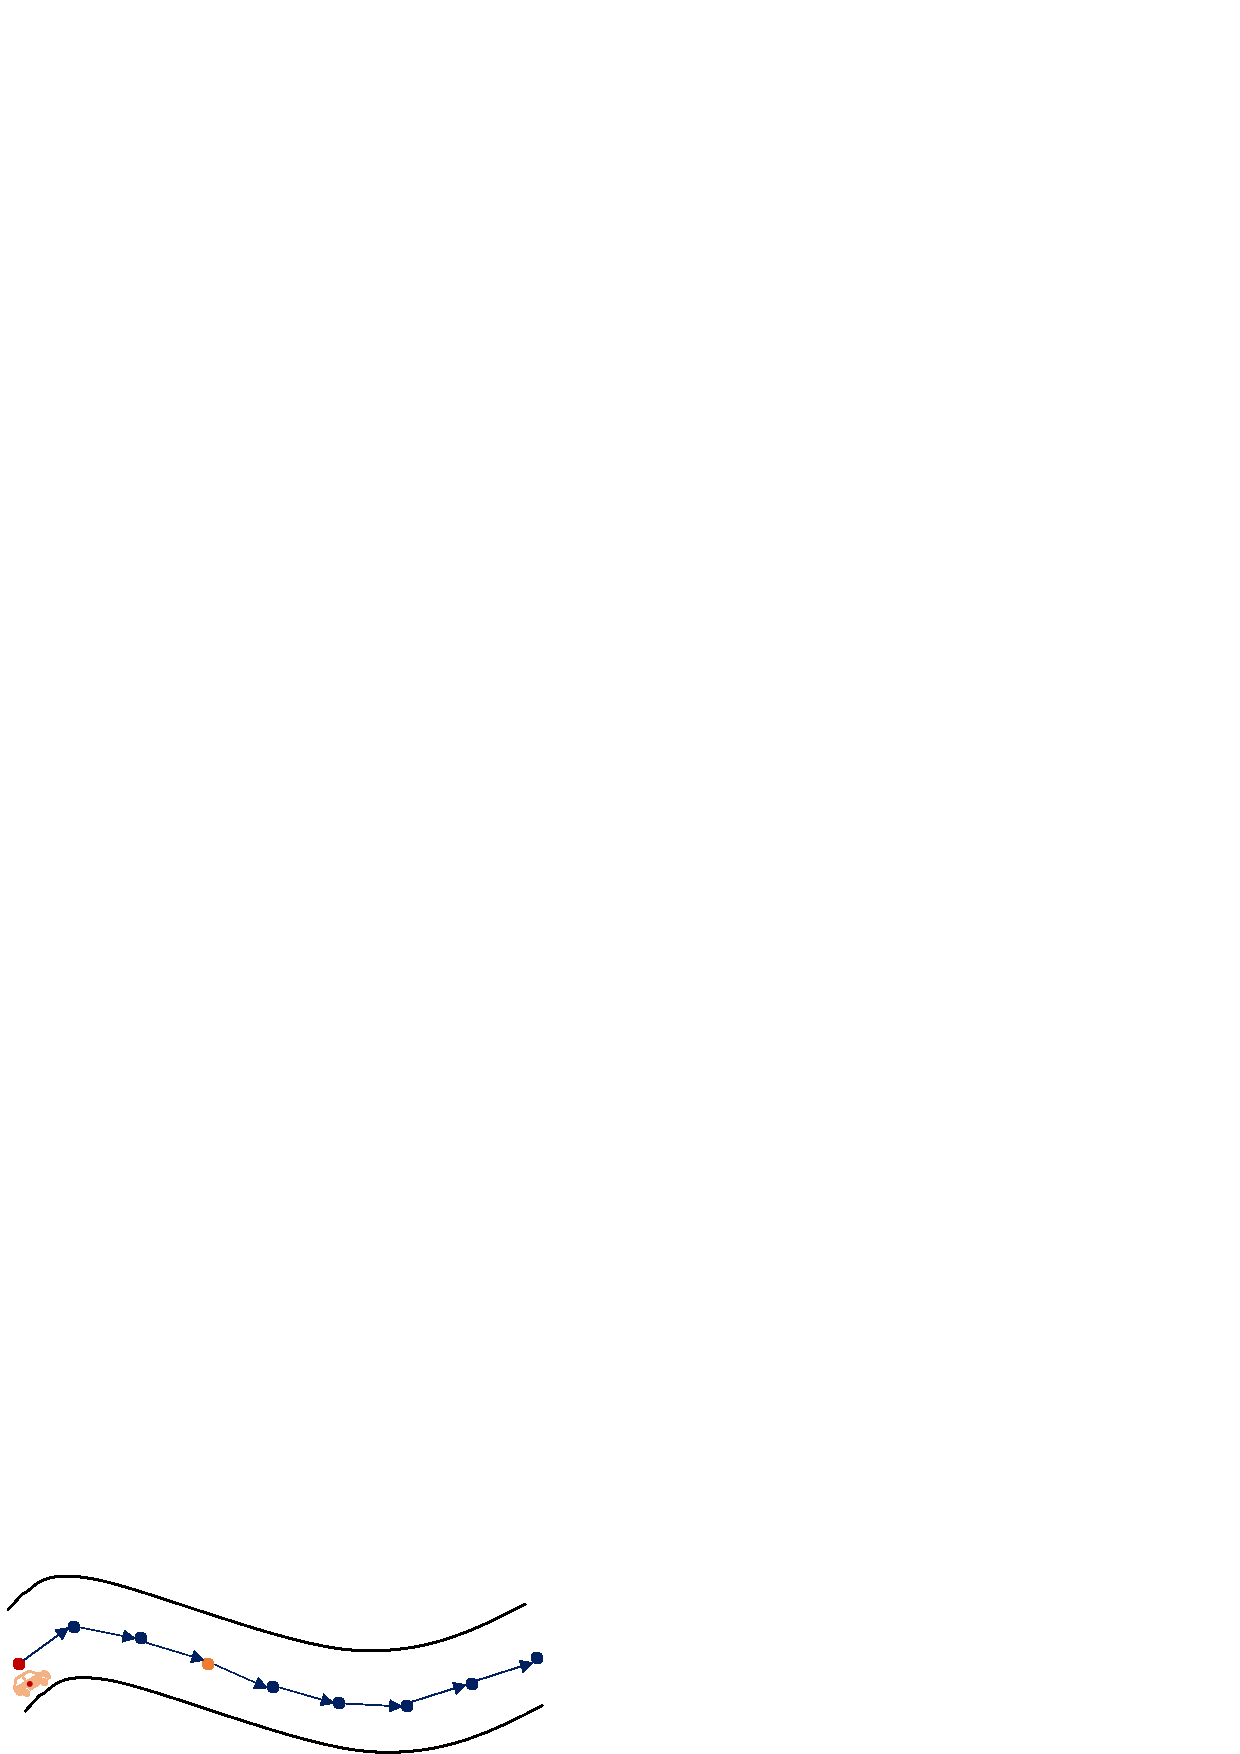
\includegraphics[width=0.45\textwidth]{figure/algExplain.png}
\caption{Preview control, strategy adopted by Matlab in Mode 1, where red dot represents the nearest way point relative to $p_i^k$, and radius value of the black circle is equal to value of preview distance, and the orange and blue dots represent target and candidate way point respectively.}
\end{figure}
\begin{algorithm}[htbp]
	\label{alg:mode1}
	\caption{Preview control}
	\LinesNumbered 
	\KwIn{Position ($p_i^k$) of vehicle $i$ at time $k$}%输入参数
	\KwOut{status of each vehicle at next time: $v$${_i^{k+1}}$, $h$$_i^{k+1}$, $p$$_i^{k+1}$, where $v$ denotes speed, and $h$ denotes orientation and $p$ denotes position}
	Find the nearest way point\,$w_n$ among the set ($W$) of all way points, and determine the target way point ($w_{target}$) based on $w_n$ and preview distance ($d$)\;
	\Begin{
		\For{$w_i\in W$}
		{ dis=$Distance(w_i,p_i^k)$\;
		\If{$dis\leq d$}
		{
			Index of $w_i$ in $W~(I_i)$\; 
			Index of $w_n$ in $W~(I_n)$\; 
			\If{$I_i\textgreater I_n$}{$w_{target}$$\longleftarrow$ $w_i$, and Equation~\ref{equ:mode1} is adpoted to calcucate outputs\;
			break.	
	}
		}
		}
	}
\end{algorithm}

\begin{figure*}[htbp]
	\begin{centering}
		\subfigure[Rectangular loop driving platoon]{
			\label{fig:physicalWaypoints}
			\includegraphics[width=0.32\textwidth]{figure/workstation.jpg}}
		\subfigure[Complete way points]{
			\label{fig:cyberWaypoints}
			\includegraphics[width=0.32\textwidth]{figure/waypointResult.png}}
		\subfigure[Platoon topology of information flow]{
			\label{fig:topology}
			\includegraphics[width=0.32\textwidth]{figure/topology.png}}
	\end{centering}
	\caption {Platooning scenario. From left to right, where \ref{fig:physicalWaypoints} demonstrates camera perspective of way points set. \ref{fig:cyberWaypoints} represents its cyber counterpart. \ref{fig:topology} describes platoon's information flow topology, where PLF topology\cite{ref:zhengyang} is adopted.}
\end{figure*}
\begin{table*}
	\centering
	\caption {Parameter explanations of Fig.\ref{fig:systemTopology} }
	\label {tab:matlab}
	\begin{tabular}{|c|c|c|c|c|}
	\hline
	\textbf{Number}&\textbf{From}&\textbf{To}&\textbf{Frequency(Hz)}&Main content \\ \hline
	\textcircled{1}&PS&Cloud&2&Real-time statuses of vehicle 1, 3 and 5  \\ \hline
	\textcircled{2}&Cloud&PS&10&Control messages for vehicle 1, 3 and 5   \\ \hline
	\textcircled{3}&CS&Cloud&10&Real-time statuses of vehicle 0, 2, 4 and 6   \\ \hline
	\textcircled{4}&Cloud&CS&10&Control messages for vehicle 0, 2, 4 and 6    \\ \hline	
	\textcircled{5}&Matlab&Cloud&10&Real-time statuses of all vehicles  \\ \hline
	\textcircled{6}&Cloud&Matlab&10&Control messages for all vehicles   \\ \hline				
	\end{tabular}
\end{table*}
\subsubsection{Obstacle Avoidance Scenario of Platoon }We design scenario of platoon obstacle avoidance for three purposes. First, we wish to prove that decision-making and motion of miniature vehicles can be effected by inexistent cloud members. Second, we wish to reflect one of the most distinguishing features of DIRS that remote perception and centralized decision-making are achievable if cloud can integrate global information. Finally, obstacle can be generated by intent captured on Hololens, which is one of the most important applications of Hololens in DIRS.

\begin{figure}
	\label{fig:obstacleAvoidance}
	\includegraphics[width=0.45\textwidth]{figure/obstacleAvoidance.png}
	\caption{Local trajectory candidates}
\end{figure}
\subsection{Result analysis}

	Figure~\ref{subsec:simulationresults} presents the experiment results. As shown in Figure~\ref{spacingHeadway} that values of spacing headway oscillate around the expected value( in green) and that the larger the distance from leading vehicle, the more significant the fluctuation phenomenon is. While Figure~\ref{speedCurve} demonstrates that when speed of leading vehicle varies in the form of square waves, speeds of following members show the same trend. Similarly, the larger the distance from leading vehicle, the more significant the overshoot phenomenon was.

\section{Conclusion and future work}
\label{sec:conclusion}
	In this study, a CAV-orientated digital twin realization system(\,DIRS) is proposed and developed to facilitate experiments containing both field and simulation validation. Besides, several novel ways are designed to support HMI. To verify effectiveness of the system, we conducted an experiment under car-following scenario, which is simple but functions as the foundation of complex ones, like platoon formation control and collaborative intersection control that we would like to conduct later. Simulation results demonstrated that DIRS is fully capable to support validation with various optional control parameters.
	
	As a customized simulation platform, several problems need to be solved along its future application: 1): scenarios or experiments could be implemented should be further enriched and evaluated to demonstrate its capability. 2): model errors and impact of time-delay to the system should be quantified, since these factors would influence performance of the system directly. 3): DIRS provides various ways to support HMI, but how to get people more involved is still challenging and needs further considerations.
\section{Acknowledgment}


\begin{thebibliography}{99}
\bibitem{ref:intro1} Wang Z, Liao X, Zhao X, et al. A digital twin paradigm: Vehicle-to-cloud based advanced driver assistance systems[C]//2020 IEEE 91st Vehicular Technology Conference (VTC2020-Spring). IEEE, 2020: 1-6.
\bibitem{ref:intro2} Liao X, Wang Z, Zhao X, et al. Cooperative Ramp Merging Design and Field Implementation: A Digital Twin Approach based on Vehicle-to-Cloud Communication[J].
\bibitem{ref:intro3} Chen Q, Wang X, Yang J, et al. Trajectory-following guidance based on a virtual target and an angle constraint[J]. Aerospace Science and Technology, 2019, 87: 448-458.
\bibitem{ref:lfq} Xu Q, Cai M, Li K, et al. Coordinated formation control for intelligent and connected vehicles in multiple traffic scenarios[J]. IET Intelligent Transport Systems, 2021, 15(1): 159-173.
\bibitem{ref:ccy} Chen C, Xu Q, Cai M, et al. A Graph-based Conflict-free Cooperation Method for Intelligent Electric Vehicles at Unsignalized Intersections[J]. arXiv preprint arXiv:2103.14290, 2021.
\bibitem{ref:taofei} Tao F, Zhang H, Liu A, et al. Digital twin in industry: State-of-the-art[J]. IEEE Transactions on Industrial Informatics, 2018, 15(4): 2405-2415.
\bibitem{ref:meth1} G. Schroeder et al., “Visualising the digital twin using web services and
augmented reality,” in Proc. IEEE 14th Int. Conf. Ind. Informat., Poitiers, France, 2016, pp. 522–527, doi: 10.1109/INDIN.2016.7819217.
\bibitem{ref:hotdec}  A. Stubbs, V. Vladimerou, A. T. Fulford, D. King, J. Strick and G. E. Dullerud, "Multivehicle systems control over networks: a hovercraft testbed for networked and decentralized control," in IEEE Control Systems Magazine, vol. 26, no. 3, pp. 56-69, June 2006, doi: 10.1109/MCS.2006.1636310.
\bibitem{ref:website} https://github.com/yangchunying123/DIRS
\bibitem{ref:engine1} Wang Z, Wu G, Boriboonsomsin K, et al. Cooperative ramp merging system: Agent-based modeling and simulation using game engine[J]. SAE International Journal of Connected and Automated Vehicles, 2019, 2(2).
\bibitem{ref:engine2} Liao X, Zhao X, Wu G, et al. A Game Theory Based Ramp Merging Strategy for Connected and Automated Vehicles in the Mixed Traffic: A Unity-SUMO Integrated Platform[J]. arXiv preprint arXiv:2101.11237, 2021.
\bibitem{ref:zhengyang} Li S E, Zheng Y, Li K, et al. An overview of vehicular platoon control under the four-component framework[C]//2015 IEEE Intelligent Vehicles Symposium (IV). IEEE, 2015: 286-291.
\end{thebibliography}
\vspace{12pt}
\color{red}
\end{document}
